\documentclass[UTF8,a4paper,11pt,fontset=fandol]{ctexart}
\usepackage{geometry}
\geometry{margin=2.2cm}
\usepackage{amsmath,amssymb,longtable,booktabs,array,hyperref,xcolor,enumitem,graphicx,float}
\hypersetup{colorlinks=true,linkcolor=blue,urlcolor=blue}
\setlist[itemize]{leftmargin=1.3em,itemsep=0.2em}
\definecolor{notegray}{RGB}{246,248,251}
\title{P11. A Spatial-Domain Coordinated Control Method for CAVs at Unsignalized Intersections Considering Motion Uncertainty\\中英双语博士精读笔记}
\author{Tong Zhao; Nikolce Murgovski; Baigen Cai; Wei ShangGuan}
\date{2025 · arXiv preprint}
\begin{document}
\maketitle

\noindent\textbf{Theme / 主题：} Spatial-domain robust trajectory planning\\
\textbf{Method family / 方法族：} Spatial-domain robust MPC / 空间域鲁棒模型预测控制\\
\textbf{PDF pages / 页数：} 15 \quad
\textbf{Relevance / 相关度：} 92/100\\
\textbf{Source / 来源：} \url{https://arxiv.org/abs/2412.04290}

\section{论文全景速览与核心贡献 / High-Level Overview \& Core Contributions}
\subsection{研究背景与痛点 / Background \& Pain Points}
这篇论文位于“Spatial-domain robust trajectory planning”方向。对你的 JSSP-based Intersection Management 课题，它回答的是高层调度、低层轨迹平滑、安全过滤或真实验证中的一个关键子问题：如何让车辆在路口少停、少冲突、少能耗，同时保持在线可执行。

The paper belongs to the theme of Spatial-domain robust trajectory planning. For a JSSP-based intersection-management thesis, it illuminates one of the key layers: scheduling, smoothing, safety filtering, or real-world validation.

\textbf{Pain point / 痛点：} Optimization-heavy; not a learned scheduler, and publication venue beyond arXiv not verified.

\subsection{核心科学问题 / Core Scientific Question}
在路径和速度存在不确定性时，如何把交叉口多类型冲突统一成可实时求解的空间域约束？

How can crossing, following, merging, and diverging conflicts be unified as real-time spatial-domain constraints under motion uncertainty?

\subsection{科学贡献 / Scientific Contributions}
\begin{itemize}
\item 方法贡献 (method contribution)：Transforms coordinated control into a spatial-domain nonlinear program with unified linear collision-avoidance constraints and real-time iteration.
\item 安全/避碰贡献 (safety contribution)：Handles crossing, following, merging, and diverging conflicts under path and speed uncertainty of HDVs.
\item 平滑/停止避免贡献 (smoothing contribution)：Generates smooth trajectories under state/control constraints, avoiding unnecessary braking where robust constraints permit.
\item 创新力度评判 (reviewer judgement)：很强：空间域建模和统一线性碰撞约束对低层 smoother 安全可行性极有价值。
\end{itemize}


\subsection{核心概念对照 / Core Concepts}
\begin{longtable}{p{0.24\linewidth}p{0.28\linewidth}p{0.40\linewidth}}
\toprule
中文概念 & English Concept & Role / 学术作用\\
\midrule
自动交叉口管理 & Autonomous Intersection Management & 把信号控制替换为车辆级调度与控制。 \\
轨迹平滑 & Trajectory Smoothing & 减少急加减速、停车和能耗峰值。 \\
安全约束 & Safety Constraints & 把碰撞风险写成距离、时间间隔或屏障函数。 \\
Spatial-domain robust MPC & 空间域鲁棒模型预测控制 & 该论文的核心方法族。 \\
\bottomrule
\end{longtable}

\section{教材式学习路径与关键截图 / Textbook-Style Study Path \& PDF Snapshots}
\subsection{学习路径 / Study Path}
\begin{itemize}
\item 第一遍先读首页截图、摘要与引言，确认研究问题和场景假设。
\item 第二遍沿着技术路线图复现模型变量、约束和求解器输入输出。
\item 第三遍逐节阅读 section deep reading，对照 PDF 截图检查公式、图表和实验。
\item 第四遍只站在审稿人视角重读实验，判断 baseline、公平性、消融和鲁棒性。
\item 最后把博士 checklist 写成自己的复现实验或论文拓展计划。
\end{itemize}


\subsection{博士阅读 Checklist / Doctoral Reading Checklist}
\begin{itemize}
\item 能否独立重写核心公式：空间域动力学与鲁棒碰撞约束 / Spatial-domain dynamics and robust collision constraints，并解释每个符号的物理意义？
\item 能否画出输入-模型-算法-控制-验证的数据流图？
\item 能否指出至少两个强假设，并说明它们在真实交通中何时失效？
\item 能否复述实验基准是否公平，指标是否覆盖效率、安全、能耗和计算时间？
\item 能否提出一个与自己 JSSP/RL/smoother 课题直接相连的拓展实验？
\end{itemize}


\subsection{关键截图讲解 / PDF Snapshot Explanation}
Screenshots are selected anchors from the local PDFs for study and parallel reading. They do not replace the original paper.

\begin{figure}[H]
\centering

\includegraphics[width=0.92\linewidth]{../../assets/P11_zhao2025spatial/01_title_and_abstract_p1.jpg}
\caption{首页与摘要 / Title and abstract page (p.1, full\_page). 这张截图用于把笔记中的抽象概念拉回原论文页面，便于你平行阅读原文、公式、图表和实验设置。 与当前课题的连接：Very strong for the smoother's feasibility and robust collision-avoidance constraints.}
\end{figure}

\begin{figure}[H]
\centering

\includegraphics[width=0.92\linewidth]{../../assets/P11_zhao2025spatial/02_modeling_or_problem_setup_p3.jpg}
\caption{建模或问题设定页 / Modeling or problem-setup page (p.3, full\_page). 这张截图用于把笔记中的抽象概念拉回原论文页面，便于你平行阅读原文、公式、图表和实验设置。 与当前课题的连接：Very strong for the smoother's feasibility and robust collision-avoidance constraints.}
\end{figure}

\begin{figure}[H]
\centering
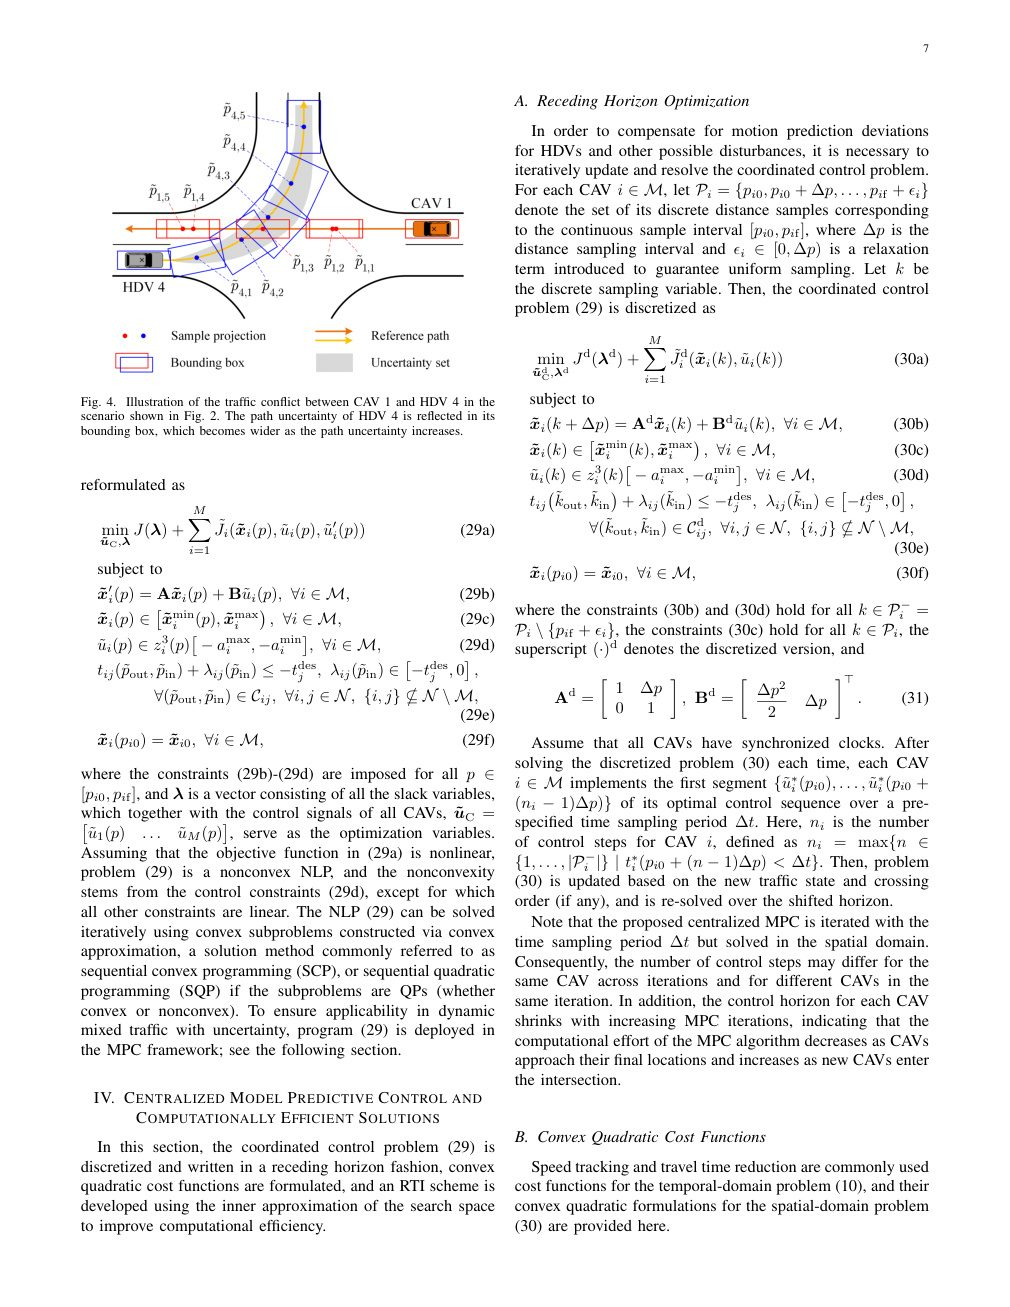
\includegraphics[width=0.92\linewidth]{../../assets/P11_zhao2025spatial/03_core_method_or_algorithm_p7.jpg}
\caption{核心方法或算法页 / Core method or algorithm page (p.7, full\_page). 这张截图用于把笔记中的抽象概念拉回原论文页面，便于你平行阅读原文、公式、图表和实验设置。 与当前课题的连接：Very strong for the smoother's feasibility and robust collision-avoidance constraints.}
\end{figure}

\begin{figure}[H]
\centering

\includegraphics[width=0.92\linewidth]{../../assets/P11_zhao2025spatial/04_experiments_or_results_p8.jpg}
\caption{实验或结果页 / Experiments or results page (p.8, full\_page). 这张截图用于把笔记中的抽象概念拉回原论文页面，便于你平行阅读原文、公式、图表和实验设置。 与当前课题的连接：Very strong for the smoother's feasibility and robust collision-avoidance constraints.}
\end{figure}

\begin{figure}[H]
\centering

\includegraphics[width=0.92\linewidth]{../../assets/P11_zhao2025spatial/05_conclusion_or_limitations_p13.jpg}
\caption{结论或局限页 / Conclusion or limitations page (p.13, figure\_crop). 这张截图用于把笔记中的抽象概念拉回原论文页面，便于你平行阅读原文、公式、图表和实验设置。 与当前课题的连接：Very strong for the smoother's feasibility and robust collision-avoidance constraints.}
\end{figure}


\section{章节精读与逐段导读 / Section-by-Section Deep Reading \& Walkthrough}
\subsection*{p.1 I. INTRODUCTION}
\textbf{章节目标 / Learning goal：} 建立研究动机：为什么传统信号控制、FCFS 或单车控制不足以处理该论文关注的交叉口协同问题。

Understand why the paper needs a new coordination method rather than a standard signal, FCFS, or single-vehicle controller.

\textbf{关键论点 / Key argument：} 这一部分通常把痛点落到 Spatial-domain robust trajectory planning：既要提高效率，又要保持安全与在线可执行。

\textbf{技术焦点 / Technical focus：} 精读时标出作者批判的 baseline、场景假设、交通参与者类型和隐含优化目标。

\textbf{审稿追问 / Reviewer question：} 作者指出的痛点是否真的需要新方法，还是可以由更强的优化器/更保守规则解决？

\subsection*{p.3 II. PROBLEM FORMULATION}
\textbf{章节目标 / Learning goal：} 把自然语言交通问题压缩为变量、状态、约束、目标函数或图结构。

Translate the traffic problem into variables, states, constraints, objectives, or graph relations.

\textbf{关键论点 / Key argument：} 本节是复现论文的核心入口，应与公式“空间域动力学与鲁棒碰撞约束 / Spatial-domain dynamics and robust collision constraints”一起读。

\textbf{技术焦点 / Technical focus：} 逐项检查车辆状态、冲突关系、控制输入、时间/空间索引和安全阈值是否定义完整。

\textbf{审稿追问 / Reviewer question：} 这些建模假设在混合交通、通信延迟、感知误差和高密度车流下是否仍成立？

\subsection*{p.4 III. M ODELING OF CONFLICT RESOLUTION CONSIDERING}
\textbf{章节目标 / Learning goal：} 承接前后章节，补充局部定义、案例或实现细节。

Recover implementation details needed for reproduction.

\textbf{关键论点 / Key argument：} 这类章节常常不是主贡献，但决定你能否真正复现方法。

\textbf{技术焦点 / Technical focus：} 检查它是否给出了参数、伪代码、场景划分或实现细节。

\textbf{审稿追问 / Reviewer question：} 跳过该节会不会导致公式或实验无法复现？

\subsection*{p.7 IV. C ENTRALIZED MODEL PREDICTIVE CONTROL AND}
\textbf{章节目标 / Learning goal：} 把自然语言交通问题压缩为变量、状态、约束、目标函数或图结构。

Translate the traffic problem into variables, states, constraints, objectives, or graph relations.

\textbf{关键论点 / Key argument：} 本节是复现论文的核心入口，应与公式“空间域动力学与鲁棒碰撞约束 / Spatial-domain dynamics and robust collision constraints”一起读。

\textbf{技术焦点 / Technical focus：} 逐项检查车辆状态、冲突关系、控制输入、时间/空间索引和安全阈值是否定义完整。

\textbf{审稿追问 / Reviewer question：} 这些建模假设在混合交通、通信延迟、感知误差和高密度车流下是否仍成立？

\subsection*{p.8 V. SIMULATION RESULTS}
\textbf{章节目标 / Learning goal：} 验证方法是否在公平基准下改善效率、安全、能耗或计算时间。

Check whether the claimed improvements are supported by fair baselines and meaningful metrics.

\textbf{关键论点 / Key argument：} 实验应与论文声称的贡献闭环：Simulation case studies; reported RTI computation reduction by orders of magnitude with small optimality loss.

\textbf{技术焦点 / Technical focus：} 重点追踪指标：求解时间、最优性损失、碰撞约束余量、通行时间、速度平滑性和不确定性敏感性。 同时检查仿真平台、交通需求和随机性设置。

\textbf{审稿追问 / Reviewer question：} 实验是否只展示平均收益，还是覆盖了高密度、异常扰动和失败案例？

\subsection*{p.10 6. The shaded space shows the motion uncertainty of HDV 4, where the X-Y}
\textbf{章节目标 / Learning goal：} 承接前后章节，补充局部定义、案例或实现细节。

Recover implementation details needed for reproduction.

\textbf{关键论点 / Key argument：} 这类章节常常不是主贡献，但决定你能否真正复现方法。

\textbf{技术焦点 / Technical focus：} 检查它是否给出了参数、伪代码、场景划分或实现细节。

\textbf{审稿追问 / Reviewer question：} 跳过该节会不会导致公式或实验无法复现？

\subsection*{p.10 1. Each CA V fulfills the speed and acceleration limits in all cases.}
\textbf{章节目标 / Learning goal：} 承接前后章节，补充局部定义、案例或实现细节。

Recover implementation details needed for reproduction.

\textbf{关键论点 / Key argument：} 这类章节常常不是主贡献，但决定你能否真正复现方法。

\textbf{技术焦点 / Technical focus：} 检查它是否给出了参数、伪代码、场景划分或实现细节。

\textbf{审稿追问 / Reviewer question：} 跳过该节会不会导致公式或实验无法复现？

\subsection*{p.13 VI. CONCLUSION AND FUTURE WORK}
\textbf{章节目标 / Learning goal：} 提炼作者承认的边界，并把它转化为博士课题的可拓展问题。

Convert acknowledged boundaries into research opportunities.

\textbf{关键论点 / Key argument：} 结论不只是总结结果，更是观察作者没有解决什么的窗口。

\textbf{技术焦点 / Technical focus：} 把 future work 与前文假设逐一对应，寻找可发表的补强点。

\textbf{审稿追问 / Reviewer question：} 如果我是审稿人，我会要求补哪一个实验、定理或消融？


\subsection{逐段式导读 / Paragraph-Level Walkthrough}
\paragraph{Opening motivation / 开篇动机段}先把作者的痛点翻译成一句博士问题：在路径和速度存在不确定性时，如何把交叉口多类型冲突统一成可实时求解的空间域约束？ 读这一段时不要急着接受动机，要追问传统 FCFS、信号灯或保守 MPC 为什么不足。

Turn the opening motivation into one doctoral-level question and test whether the paper truly needs a new method.

\paragraph{Assumption and setting / 假设与场景段}把车辆类型、通信条件、路口类型和动力学假设列成表。该文的关键边界包括：车辆路径可用空间坐标参数化。；不确定性集合边界可估计且不严重失真。；集中式求解器可在控制周期内完成。

List vehicle type, communication, intersection setting, and dynamics assumptions before reading the equations.

\paragraph{Model and notation / 模型与符号段}围绕核心公式“空间域动力学与鲁棒碰撞约束 / Spatial-domain dynamics and robust collision constraints”复写符号表，确认每个变量是决策变量、状态变量、参数还是约束阈值。

Rewrite the symbol table around the core formulation and classify variables as states, decisions, parameters, or constraints.

\paragraph{Algorithm mechanism / 算法机制段}把算法读成一条数据流：输入交通状态，执行 Transforms coordinated control into a spatial-domain nonlinear program with unified linear collision-avoidance constraints and real-time iteration.，输出可执行通行/控制决策，并检查安全接口。

Read the algorithm as a dataflow from traffic state to executable sequence/control decision, with explicit safety interfaces.

\paragraph{Experiment and evidence / 实验证据段}不要只看作者报告的提升，要检查基准、公平性和指标。本文验证描述为：Simulation case studies; reported RTI computation reduction by orders of magnitude with small optimality loss.

Go beyond reported gains and inspect baselines, fairness, metrics, and computation time.

\paragraph{Reviewer synthesis / 审稿式总结段}最后把贡献拆成可发表与需补强两部分。对你课题最直接的用途是：Very strong for the smoother's feasibility and robust collision-avoidance constraints.

Separate publishable contribution from missing evidence, then connect the result to your own thesis architecture.


\section{技术路线图与贡献量评估 / Technical Route \& Contribution Matrix}
\begin{longtable}{p{0.08\linewidth}p{0.24\linewidth}p{0.58\linewidth}}
\toprule
Step & Stage / 阶段 & Content / 内容\\
\midrule
1 & 输入 / Input & 车辆状态、路径/车道、交通需求、信号或协同信息。 \\
2 & 建模 / Modeling & 空间域动力学与鲁棒碰撞约束 / Spatial-domain dynamics and robust collision constraints \\
3 & 核心求解 / Core solver & Transforms coordinated control into a spatial-domain nonlinear program with unified linear collision-avoidance constraints and real-time iteration. \\
4 & 安全接口 / Safety interface & Handles crossing, following, merging, and diverging conflicts under path and speed uncertainty of HDVs. \\
5 & 平滑与效率 / Smoothing and efficiency & Generates smooth trajectories under state/control constraints, avoiding unnecessary braking where robust constraints permit. \\
6 & 验证 / Validation & Simulation case studies; reported RTI computation reduction by orders of magnitude with small optimality loss. \\
\bottomrule
\end{longtable}

\begin{longtable}{p{0.34\linewidth}p{0.14\linewidth}p{0.42\linewidth}}
\toprule
Dimension / 维度 & Score & Comment / 评语\\
\midrule
理论贡献 / Theoretical contribution & 4/5 & 空间域动力学与鲁棒碰撞约束 / Spatial-domain dynamics and robust collision constraints \\
算法贡献 / Algorithmic contribution & 4/5 & Transforms coordinated control into a spatial-domain nonlinear program with unified linear collision-avoidance constraints and real-time iteration. \\
实验贡献 / Experimental contribution & 3/5 & Simulation case studies; reported RTI computation reduction by orders of magnitude with small optimality loss. \\
工程贡献 / Engineering contribution & 4/5 & Handles crossing, following, merging, and diverging conflicts under path and speed uncertainty of HDVs. \\
博士课题价值 / PhD relevance & 5/5 & Very strong for the smoother's feasibility and robust collision-avoidance constraints. \\
\bottomrule
\end{longtable}

\section{理论方法论深度解构 / Methodology \& Theoretical Framework}
\subsection{问题数学建模 / Mathematical Formulation}
\textbf{空间域动力学与鲁棒碰撞约束 / Spatial-domain dynamics and robust collision constraints}
\[
\frac{dt_i}{ds}=\frac{1}{v_i(s)},\quad \min_{u_i(s)}\sum_i\int \left(w_t\frac{1}{v_i(s)}+w_u u_i(s)^2\right)ds,\quad h_{ij}(s,\Delta)\ge d_{safe}
\]
\begin{longtable}{p{0.16\linewidth}p{0.25\linewidth}p{0.25\linewidth}p{0.25\linewidth}}
\toprule
Symbol / 符号 & 含义 & Meaning & Role / 建模作用\\
\midrule
s & 空间路径坐标 & spatial path coordinate & 把时间规划转成沿路径规划 \\
v\_i(s) & 空间域速度 & speed over path coordinate & 决定到达时间和安全间隔 \\
h\_ij & 车辆 i,j 的冲突间隔函数 & conflict-separation function & 统一多种冲突类型 \\
Delta & 运动不确定性 & motion uncertainty & 路径/速度误差集合 \\
d\_safe & 安全距离阈值 & safe-distance threshold & 鲁棒约束下界 \\
\bottomrule
\end{longtable}

\subsection{核心算法架构 / Core Algorithm Layout}
论文把轨迹规划从时间域转为空间域，针对 crossing/following/merging/diverging 构造统一线性化安全约束，再用集中式 MPC 和实时迭代求解，以较小最优性损失换取计算速度。

The method transforms coordination into a spatial-domain nonlinear program, linearizes unified collision-avoidance constraints, and solves it with real-time MPC iterations.

\subsection{收敛性、稳定性或实时性 / Convergence, Stability, Real-Time Feasibility}
鲁棒性来自显式不确定集合与安全约束，实时性来自空间域简化和 RTI。相比纯学习策略，这类 smoother 更容易给审稿人安全信心。

Robustness comes from explicit uncertainty sets and safety constraints; RTI makes the spatial-domain MPC viable online.

\subsection{潜在假设与边界条件 / Assumptions \& Boundary Conditions}
\begin{itemize}
\item 车辆路径可用空间坐标参数化。
\item 不确定性集合边界可估计且不严重失真。
\item 集中式求解器可在控制周期内完成。
\end{itemize}


\section{实验验证与结果评判 / Experimental Validation \& Result Evaluation}
\textbf{Baselines \& Environment / 基准与环境：} 时间域 MPC、非鲁棒控制、保守安全间隔策略和不同 RTI 近似。

\textbf{Validation / 验证：} Simulation case studies; reported RTI computation reduction by orders of magnitude with small optimality loss.

\textbf{Metrics / 指标：} 求解时间、最优性损失、碰撞约束余量、通行时间、速度平滑性和不确定性敏感性。

\textbf{Ablation / 消融：} 很适合做鲁棒半径、RTI 次数、统一约束 vs 分类型约束的消融。

\textbf{Reviewer reading / 审稿式阅读提醒：} 阅读实验时不要只看平均值；应检查交通密度、车流方向、随机种子、失败案例和计算耗时。For doctoral reading, inspect density regimes, demand patterns, random seeds, failure cases, and computation time rather than only mean improvements.

\subsection{图表阅读线索 / Figure and Table Reading Cues}
PDF extraction detected approximately 41 figure references and 5 table references. Exact captions remain in the original PDF; the bilingual cues below tell you what to inspect first.

\begin{longtable}{p{0.24\linewidth}p{0.30\linewidth}p{0.36\linewidth}}
\toprule
图表名称 & Figure/Table Name & Reading focus / 阅读重点\\
\midrule
系统框架图 & system framework diagram & 先确认输入、决策层、控制层和安全约束之间的数据流。 \\
控制框架/轨迹曲线图 & control-framework or trajectory-profile plots & 关注约束激活位置、速度/加速度曲线和安全裕度是否平滑。 \\
实验指标对比图表 & experimental metric comparison plots/tables & 重点看平均值之外的密度变化、失败场景、计算时间和方差。 \\
\bottomrule
\end{longtable}

\section{审稿人视角：批判性思考与未来方向 / Critical Thinking \& Future Directions}
\subsection{论文局限性 / Limitations \& Weaknesses}
\begin{itemize}
\item 优化问题仍可能在大规模车辆数下变重。
\item 不确定集合若估计过小会失去安全性，过大则过于保守。
\item 高层排序/优先级选择不是主要贡献。
\end{itemize}


\subsection{博士课题拓展点 / Research Extensions for PhD}
\begin{itemize}
\item 将 JSSP 调度输出作为 MPC 的目标时间或优先级约束。
\item 用学习模型预测不确定集合大小，实现自适应鲁棒性。
\item 把空间域安全约束封装成调度动作可行性检查器。
\end{itemize}


\subsection{如何服务当前课题 / Use in This Project}
Very strong for the smoother's feasibility and robust collision-avoidance constraints.

\section{交互式可视化与 PDF 排版蓝图 / Interactive Visualization \& PDF Layout Blueprint}
\textbf{动态参数 / Parameter：} 不确定性半径 / Uncertainty radius, range [0.0, 3.0] m.

半径越大，安全裕度越高但轨迹越保守、延误越大。

A larger uncertainty radius improves safety margin but increases conservatism.

\subsection{HTML 结构化布局建议 / HTML Structuring}
\begin{itemize}
\item 顶部固定 metadata bar：题名、作者、年份、主题、PDF 页数。
\item 左侧目录/section navigator，右侧为五大精读模块。
\item 公式卡片使用 <pre> 或 LaTeX block，紧跟符号表。
\item 审稿人批注用 reviewer-note block，博士拓展用 research-idea list。
\item 交互参数用 input[type=range] + canvas 曲线，打印 PDF 时隐藏交互控件但保留解释。
\end{itemize}


\section{来源锚点与逐节阅读路径 / Source Anchors \& Section-by-Section Reading Map}
\begin{longtable}{p{0.14\linewidth}p{0.76\linewidth}}
\toprule
Page & Extracted heading\\
\midrule
p.1 & I. INTRODUCTION \\
p.3 & II. PROBLEM FORMULATION \\
p.8 & V. SIMULATION RESULTS \\
\bottomrule
\end{longtable}

\paragraph{p.1 I. INTRODUCTION}定位问题背景、研究缺口和为什么现有保守/非协同方法不足。 / Frames the motivation, research gap, and limits of conservative or non-cooperative methods.

\paragraph{p.3 II. PROBLEM FORMULATION}把交通交互转写为状态、约束、目标或图结构，是精读时最应复现的部分。 / Defines states, constraints, objectives, or graph structures; this is the section to reproduce carefully.

\paragraph{p.4 III. M ODELING OF CONFLICT RESOLUTION CONSIDERING}作为局部论证段落阅读，关注它如何服务主问题。 / Read as a local argument and ask how it supports the main question.

\paragraph{p.7 IV. C ENTRALIZED MODEL PREDICTIVE CONTROL AND}把交通交互转写为状态、约束、目标或图结构，是精读时最应复现的部分。 / Defines states, constraints, objectives, or graph structures; this is the section to reproduce carefully.

\paragraph{p.8 V. SIMULATION RESULTS}检验方法是否真的改善效率、安全或能耗；要关注基准是否公平。 / Tests efficiency, safety, or energy claims; inspect whether baselines are fair.

\paragraph{p.10 6. The shaded space shows the motion uncertainty of HDV 4, where the X-Y}作为局部论证段落阅读，关注它如何服务主问题。 / Read as a local argument and ask how it supports the main question.

\paragraph{p.10 1. Each CA V fulfills the speed and acceleration limits in all cases.}作为局部论证段落阅读，关注它如何服务主问题。 / Read as a local argument and ask how it supports the main question.

\paragraph{p.13 VI. CONCLUSION AND FUTURE WORK}总结贡献和未来方向，也常暴露作者承认的边界条件。 / Summarizes contributions and often reveals author-recognized boundaries.


\end{document}
